\chapter{GNSS Software Defined Receiver Architecture}
Since 1993, the Global Positioning System (GPS) has provided users with capable hardware to determine their global position within seconds and in recent developments, a centimeter-level position error. GPS can be explained in 3 components: the satellite vehicles in space, control and transmission of signals, and the receiver processing component.

GPS satellites have undergone multiple improvements and upgrades since the first satellites were launched in 1978. These versions of satellites are based on their \textit{block}. Currently, Block III is the most advanced satellite orbiting Earth today. Early versions (Block I) of GPS satellites were used mainly for development and did not transmit signals to the public. Lessons learned from the Block I satellites were fully integrated into the Block II GPS satellites, where GPS became fully operational in 1993. While there were many subtle differences between Block I and Block II satellites, the most important difference is that these new satellites broadcasted a signal on 2 frequencies, coined \textit{L1}, \textit{L2}, and \textit{L2c}, where \textit{L2c} is intended for civilian use. Modern day Block III satellites transmit their signal on the same frequencies that Block II satellites have, with the addition of \textit{L5}. Table provides the frequencies that signals are transmitted on.

\begin{table}[h!]\label{tbl:GPSfreq}
    \centering
    \begin{tabular}{lc}
        \toprule
        \textbf{Name} & \textbf{Frequency [Mhz]} \\
        \midrule
        \textit{L1}   & \(1575.42\)              \\
        \textit{L2}   & \(1227.60\)              \\
        \textit{L2c}  & \(1227.60\)              \\
        \textit{L5}   & \(1176.45\)              \\
        \bottomrule
    \end{tabular}
\end{table}
%% Background/Introduction

\section{Front End}
The signals received by an antenna must be down converted and digitized before the processing of the signal can take place. The \textit{Front End} of the receiver performs this conversion through a series of amplifiers, filters, and a Analog-to-Digital Converter (ADC). First, a signal is received by a Right-Hand Circularly Polarized (RHCP) antenna. The antenna can be passive, but for scenarios where long cables are used, a powered, active antenna may be necessary. Because of the low received signal power that GNSS constellations provide, the signal is amplified through a series of Low Noise Amplifiers (LNA) and Band Pass Filters (BPF). The LNA raise the power of the received GPS signal and the BPF act as a first-step in removing non-GPS signals from processing. The last stage is passing the continuous received signal through the ADC where the signal is converted to digitized samples at a frequency of the receiver-embedded oscillator. The oscillator is filtered using a phase lock loop, described later. Table~\ref{tbl:clocks} provides a description of the clock typically utilized on GNSS hardware receivers.

\begin{table}[!ht]\label{tbl:clocks}
    \caption{Typical clocks embedded on hardware GNSS receivers.}
    \centering
    \begin{tabular}{cccc}
        \toprule
        Name                        & Abbreviation & Application \\
        \midrule
        Oxidized Crystal Oscillator & OCXO         &             \\
        Oxidized Crystal Oscillator & OCXO         &             \\
        Oxidized Crystal Oscillator & OCXO         &             \\
        Oxidized Crystal Oscillator & OCXO         &             \\
        \bottomrule
    \end{tabular}
\end{table}

The purpose in this mixing process is to transform the signal into a more manageable intermediate frequency while still maintaining the same modulation and Doppler applied to the signal. Figure~\ref{fig:frontend} describes the process on converting the analog, continuous signal into a discrete, digitized IF signal in block diagram form.

\begin{figure}[!ht]\label{fig:frontend}
    \centering
    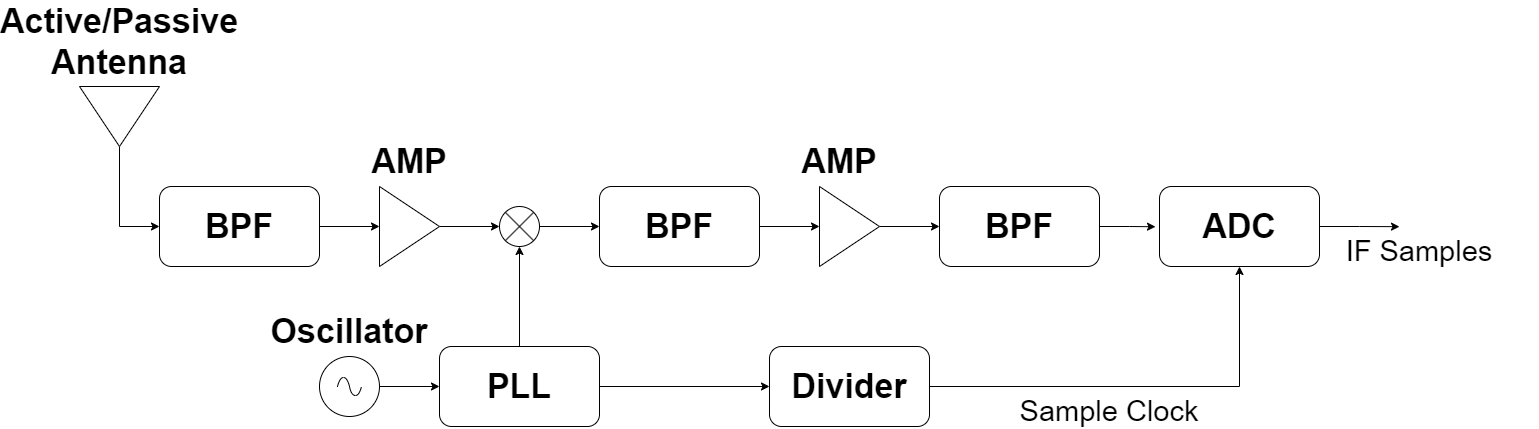
\includegraphics[width=\linewidth]{Figures/frontend.drawio.png}
    \caption{Block diagram of a software defined receiver front end}
\end{figure}

\section{Acquisition}
Once the received signals are converted to a discrete, continuous form, the receiver will determine which satellites are transmitting and in-view. Acquisition correlates local replicas of a signal with the received data. In order for there to be a large correlation magnitude, pseudo-random number (PRN) codes must be within 1-chip and the frequency of the carrier wave must also be within 250 hertz of the true frequency. Correlation with the carrier frequency can be difficult due to the trajectory of the satellite, and even more difficult if the collection perform is also moving. The motion of the satellites with respect to the receiver bring a change to the carrier frequency known as the Doppler shift. For the algorithms in acquisition to successfully determine which satellites are in-view of the receiver, it is beneficial to correlate with each satellite for the specified constellation, at each code offset, and at a wide range of carrier frequency offsets.

A modern, ubiquitous approach to correlating the local replica signals with the received data is using a Parallel Code Phase Search (PCPS) algorithm in which the correlations occur in the frequency domain~\cite{scottRapidSignalAcquisition}. PCPS parallelizes the PRN code offset search space by converting the space from the time to frequency domain. This process is shown in Figure~\ref{fig:PCPS}.

\begin{figure}[!ht]\label{fig:PCPS}
    \centering
    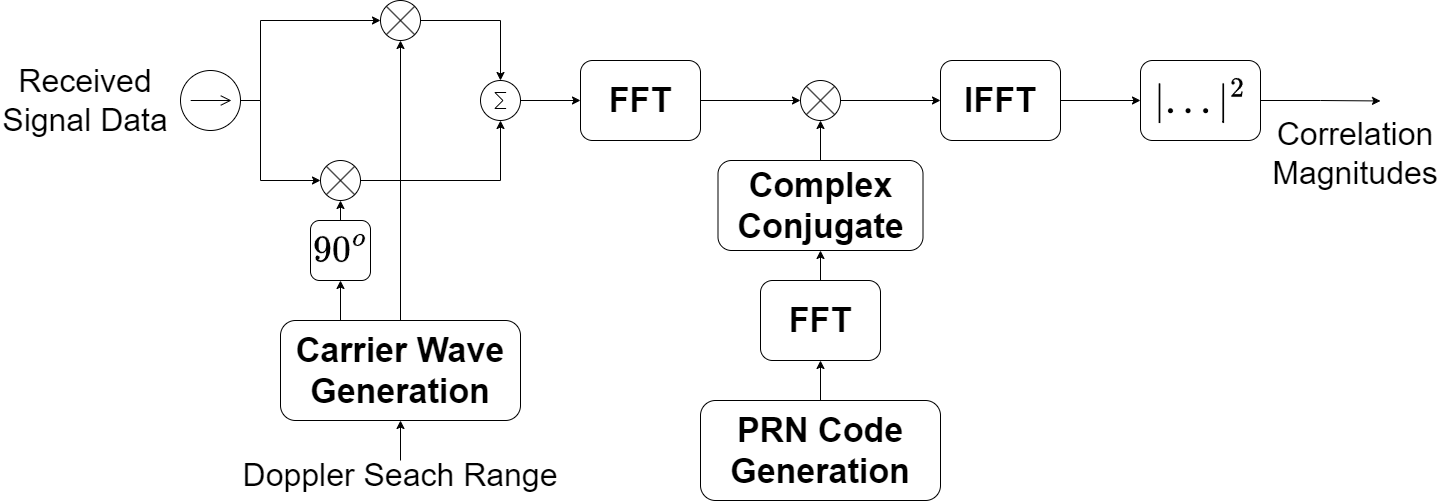
\includegraphics[width=\linewidth]{Figures/PCPS.drawio.png}
    \caption{Block diagram of the PCPS acquisition algorithm applied to GPS L1 C/A signal modulation.}
\end{figure}

To start, the local replicas of the carrier wave are multiplied with the received data across both inphase and quadrature channels in the complex number space. These resulting multiplications are summed together and passed through a Fast-Fourier Transform (FFT) to convert the vectors into the frequency domain. The second step involves converting the PRN codes of the satellites within the specified constellation to the frequency domain and then applying the complex conjugate to frequency-based, PRN vectors. Multiplying the PRN replicas with the transformed carrier replicas provides the user with an auto-correlation in the frequency domain. To appreciate the correlation magnitudes, the output is passed though an Inverse FFT, converting the correlation values from a frequency domain, complex vector to a time domain, real vector. The last step requires squaring the absolute value of this vector and then processing the next satellite until all satellites in the constellation are processed. If a correlation exceeds a certain magnitude, its location in the matrix of correlations indicates the estimated PRN code delay and Doppler shift carrier frequency for that particular satellite. The resolution of the PCPS algorithm greatly depends on the grid of Doppler search bins; for a static receiver processing GPS L1 C/A transmissions, a typical resolution is \(-15,000\) to \(15,000\) Hertz in bins of \(500\) Hertz.

\section{Tracking}
Acquisition provides initial estimates of code delay and carrier frequency for each satellite that is in-view of the receiver. However, because of the motion of the satellites and the receiver (if not static), the delays of the code and changes in the carrier frequencies must continue to be estimated. Tracking performs this process by opening a channel for each in-view satellite. For the duration of the recording, a number of algorithms within tracking continue to correlate the local receiver replica with the received signal data. For scalar tracking, Figure~\ref{fig:scalartracking} describes the flow of how these algorithms produce accurate code replicas for the receiver to calculate satellite PVT solutions.

\begin{figure}[!ht]\label{fig:scalartracking}
\centering
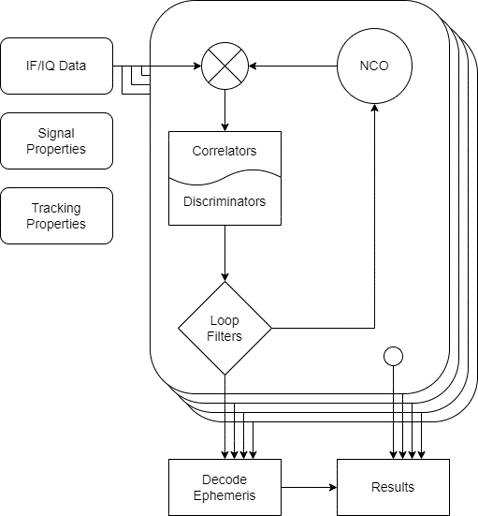
\includegraphics[width=0.5\linewidth]{Figures/scalartracking.png}
\caption{Flow diagram of scalar tracking algorithms.}
\end{figure}

\subsection{Correlators}
\subsection{Discriminators and Loop Filters}

\section{Navigation Algorithms}
\subsection{GNSS Measurements}
\subsection{Open-Loop Architectures}
\subsection{Vector Tracking}

\section{Conclusions}